\subsection{Introduction}
This is an attempt to understand of some of the most frequently-used machine learning methods by using just base Python and numpy.

t-Stochastic Neighbourhood Embedding is a dimensionality reduction algorithm. This means we can take some data that lives in a high-dimensional space (such as images, which usually consist of thousands of pixels), and visualise it in a lower-dimensional space. This is desirable, as humans are much better at understanding data when it is presented in a two- or three-dimensional space.

\subsection{SNE}
t-distributed Stochastic Neighbour Embedding, or t-SNE, was developed by Geoffrey Hinton and Laurens van der Maaten in \hyperlink{http://www.jmlr.org/papers/volume9/vandermaaten08a/vandermaaten08a.pdf}{this paper}. This appendix will just cover the SNE part.

\subsubsection{P matrix}

Given a dataset $X$ with $N$ data points and $D$ dimensions, the aim is to reduce it to $d$ dimensions: e.g. $d=2$ without losing generality. SNE converts the euclidean distance between data points to conditional probabilities of likelihood to be a neighbour.

$$ P_{j|i}=\frac{exp(-||x_i - x_j||^2 / 2\sigma^2_i)}{\sum_{k\neq i}^kexp(-||x_i - x_k||^2 / 2\sigma^2_i)} $$

This is, the probability of point $x_j$ to be a neighbour of point $x_i$ is proportional to de distance between this two points. $\sigma$ will be explained later as well as the denominator.

\emph{Note}: $p_{i|i}=0$ for all $i$ since it is irrelevant how much of a neighbour each point is with itself.

\subsubsection{Q matrix}
The $Q$ matrix is a $N\times2$ dimensional matrix, the output of t-SNE and the 2D representation of $X$.

$$ Q_{j|i}=\frac{exp(-||x_i - x_j||^2)}{\sum_{k\neq i}^kexp(-||x_i - x_k||^2)} $$

\subsubsection{KL divergence}
The overall goal is to get points $q_i$ such that the conditional probability distribution $q_i$ is similar to $p_i$. This is achieved by minimising a cost function: the \hyperlink{https://en.wikipedia.org/wiki/Kullback-Leibler_divergence}{Kullback–Leibler divergence} or KLD between these two distributions. KLD or $C$ is defined as follows:

$$ C = \sum_i KLD(P_i||Q_i) = \sum_i \sum_j P_{j,i} \log(\frac{P_{j|i}}{Q_{j|i}}) $$

The function will be minimised with \hyperlink{https://en.wikipedia.org/wiki/Gradient_descent}{gradient descent}. This will be explained later. To calculate the negative squared distances:
\begin{lstlisting}[language=Python]
def neg_squared_euc_dists(X):
    sum_X = np.sum(np.square(X), 1)
    D = np.add(np.add(-2 * np.dot(X, X.T), sum_X).T, sum_X)
    return -D
\end{lstlisting}

It returns an $N\times N$ matrix that contain the euclidean distances for all $x_i$ and $x_j$.

Also, I will need the softmax function for the denominator of the formulas for matrices $P$ and $Q$:
\begin{lstlisting}[language=Python]
def softmax(X, diag_zero=True):

    # Subtract max to scale
    e_x = np.exp(X - np.max(X, axis=1).reshape(-1, 1))

    # We usually want diagonal probabilities to be 0
    if diag_zero:
        np.fill_diagonal(e_x, 0.)

    # Add a tiny constant to avoid log problems
    e_x = e_x + 1e-16

    return e_x / e_x.sum(axis=1).reshape(-1, 1)
\end{lstlisting}

To get the matrix $P$:
\begin{lstlisting}[language=Python]
def get_P(distances, sigmas=None):
    """Convert a distances matrix to a matrix of probabilities."""
    if sigmas is not None:
        two_sig_sq = 2. * np.square(sigmas.reshape((-1, 1)))
        return softmax(distances / two_sig_sq)
    else:
        return softmax(distances)
\end{lstlisting}

\subsubsection{Perplexity}
In the previous code snippet, the sigmas argument should be an N-length vector containing each of the $\sigma_i$. This is achieved with the \hyperlink{https://en.wikipedia.org/wiki/Perplexity}{perplexity}. The perplexity of any of the rows $P_i$ of the conditional probabilities matrix $P$ is defined as:
$$ Perp(P_i) = 2^{H(P_i)}$$

Where $H(P_i)$ is the \href{https://en.wiktionary.org/wiki/Shannon_entropy}{Shannon entropy} of $P_i$ in bits:
$$ H(P_i) = - \sum p_{j|i} \log_2 (p_{j|i}) $$

In SNE, perplexity usually has a value between 5 and 50\footnote{\url{https://scikit-learn.org/stable/modules/generated/sklearn.manifold.TSNE.html}}. We then set each $\sigma_i$ such that for each row of $P$, the perplexity of that row is equal to our desired perplexity, the parameter we set.

\emph{Note}: Probability distributions with high entropy (and therefore high perplexity) are relatively flat: elements have similar probabilities. In SNE, high perplexity makes the $P_{j|i}$ similar to each other, the probability of being a neighbour is similar for all reasonably close points. The larger the perplexity, the larger the $\sigma_i$ we divide by, the closer the probability distribution gets to having all probabilities equal to just 1/N. This is why perplexity is set to the number of neighbours we believe each point has\footnote{\url{https://scikit-learn.org/stable/modules/generated/sklearn.manifold.TSNE.html}}.

To ensure the perplexity of each row of $P$, $Perp(Pi)$, is equal to the desired perplexity, it is required a binary search over each $\sigma_i$ until $Perp(Pi)$ is close enough to the desired perplexity. This is possible because $Perp(Pi)$ is a \hyperlink{https://en.wikipedia.org/wiki/Monotonic_function}{monotonically increasing function} of $\sigma_i$.

The binary search function is:
\begin{lstlisting}[language=Python]
def binary_search(eval_fn, target, tol=1e-10, max_iter=10000, lower=1e-20, upper=1000.):
    for i in range(max_iter):
        guess = (lower + upper) / 2.
        val = eval_fn(guess)
        if val > target:
            upper = guess
        else:
            lower = guess
        if np.abs(val - target) <= tol:
            break
    return guess
\end{lstlisting}

To find the $\sigma_i$ it is necessary to pass an \emph{eval\_fn} to \emph{binary\_search} function that takes a given $\sigma_i$ as its argument and returns the perplexity of $P_i$ with that $\sigma_i$.


The \emph{find\_optimal\_sigmas} function below does exactly this to find all $\sigma_i$. It takes a matrix of negative euclidean distances and a target perplexity. For each row of the distances matrix, it performs a binary search over possible values of $\sigma_i$ until finding that which results in the target perplexity. It then returns a \texttt{numpy} vector containing the optimal $\sigma_i$.

\begin{lstlisting}[language=Python]
def calc_perplexity(prob_matrix):
    entropy = -np.sum(prob_matrix * np.log2(prob_matrix), 1)
    perplexity = 2 ** entropy
    return perplexity

def perplexity(distances, sigmas):
    return calc_perplexity(calc_prob_matrix(distances, sigmas))

def find_optimal_sigmas(distances, target_perplexity):
    sigmas = [] 
    # For each row of the matrix (each point in our dataset)
    for i in range(distances.shape[0]):
        # Make fn that returns perplexity of this row given sigma
        eval_fn = lambda sigma: \
            perplexity(distances[i:i+1, :], np.array(sigma))
        # Binary search over sigmas to achieve target perplexity
        correct_sigma = binary_search(eval_fn, target_perplexity)
        # Append the resulting sigma to our output array
        sigmas.append(correct_sigma)
    return np.array(sigmas)
\end{lstlisting}

\subsubsection{Symmetric SNE}

Now, it is possible to find a 2D representation $Y$ by descending the gradient of the cost $C$ with respect to $Y$ until convergence. The gradient of SNE is more complicated to implement so in this report it will be used the Symmetric SNE. Symmetric SNE was described as 'just as good' alternative to tSNE.

\textbf{Difference}: Symmetric SNE minimises a KL divergence over the \emph{joint} probability distributions with entries $p_{i,j}$ and $q_{i,j}$, as opposed to conditional probabilities $p_{i|j}$ and $q_{i|j}$. With the joint distribution, each $q_{i,j}$ is given by:

$$ Q_{j|i}=\frac{exp(-||x_i - x_j||^2)}{\sum_{k\neq l}^kexp(-||x_k - x_l||^2)} $$

This is just like the softmax in the denominator we had before, except now the normalising term in the denominator is summed over the entire matrix $l$, rather than just the current row $i$.

To avoid problems related to outlier $X$ points:
$$ p_{ij}= \frac{p_{i|j} + p_{j|i}}{2N}$$

The code:
\begin{lstlisting}[language=Python]
def q_joint(Y):
    # Get the distances from every point to every other
    distances = neg_squared_euc_dists(Y)
    # Take the elementwise exponent
    exp_distances = np.exp(distances)
    # Fill diagonal with zeroes so q_ii = 0
    np.fill_diagonal(exp_distances, 0.)
    # Divide by the sum of the entire exponentiated matrix
    return exp_distances / np.sum(exp_distances), None


def p_conditional_to_joint(P):
    return (P + P.T) / (2. * P.shape[0])
    
def p_joint(X, target_perplexity):
    # Get the negative euclidian distances matrix for our data
    distances = neg_squared_euc_dists(X)
    # Find optimal sigma for each row of this distances matrix
    sigmas = find_optimal_sigmas(distances, target_perplexity)
    # Calculate the probabilities based on these optimal sigmas
    p_conditional = calc_prob_matrix(distances, sigmas)
    # Go from conditional to joint probabilities matrix
    P = p_conditional_to_joint(p_conditional)
    return P
\end{lstlisting}

\subsubsection{Gradient descent SNE}
After differencing the KLD, gradient descent is used to update the i'th row of our low dimensional representation $Y$:
$$ G = \frac{\partial C}{\partial y_i} = 4\sum_j (p_{ij} - q_{ij}) (y_i - y_j)$$

\begin{lstlisting}[language=Python]
def symmetric_sne_grad(P, Q, Y, _):
    pq_diff = P - Q  # NxN matrix
    pq_expanded = np.expand_dims(pq_diff, 2)  #NxNx1
    y_diffs = np.expand_dims(Y, 1) - np.expand_dims(Y, 0)  #NxNx2
    grad = 4. * (pq_expanded * y_diffs).sum(1)  #Nx2
    return grad
\end{lstlisting}

In this function, G is an $N\times2$ matrix whose i’th row is $\partial C / \partial y_i$

Afterwards, update the $y_i$ row of the $Y$ matrix:
$$Y^t_i = Y_i^{t-1} - \mu \frac{\partial C}{\partial y_i}$$

The update of the gradient descent has to be done iteratively:

\begin{lstlisting}[language=Python]
def estimate_sne(X, y, P, rng, num_iters, q_fn, grad_fn, learning_rate, momentum, plot):

    # Initialise our 2D representation
    Y = rng.normal(0., 0.0001, [X.shape[0], 2])

    # Initialise past values (used for momentum)
    if momentum:
        Y_m2 = Y.copy()
        Y_m1 = Y.copy()

    # Start gradient descent loop
    for i in range(num_iters):

        # Get Q and distances (distances only used for t-SNE)
        Q, distances = q_fn(Y)
        # Estimate gradients with respect to Y
        grads = grad_fn(P, Q, Y, distances)

        # Update Y
        Y = Y - learning_rate * grads
        if momentum:  # Add momentum
            Y += momentum * (Y_m1 - Y_m2)
            # Update previous Y's for momentum
            Y_m2 = Y_m1.copy()
            Y_m1 = Y.copy()

        # Plot sometimes
        if plot and i % (num_iters / plot) == 0:
            categorical_scatter_2d(Y,
            y,
            alpha=1.0,
            ms=6,
            show=True,
            figsize=(9, 6))

    return Y
\end{lstlisting}

\newpage
\subsubsection{Results: MNIST dataset}

\begin{figure}[H]
\centering
\subfloat[0 iterations]{
  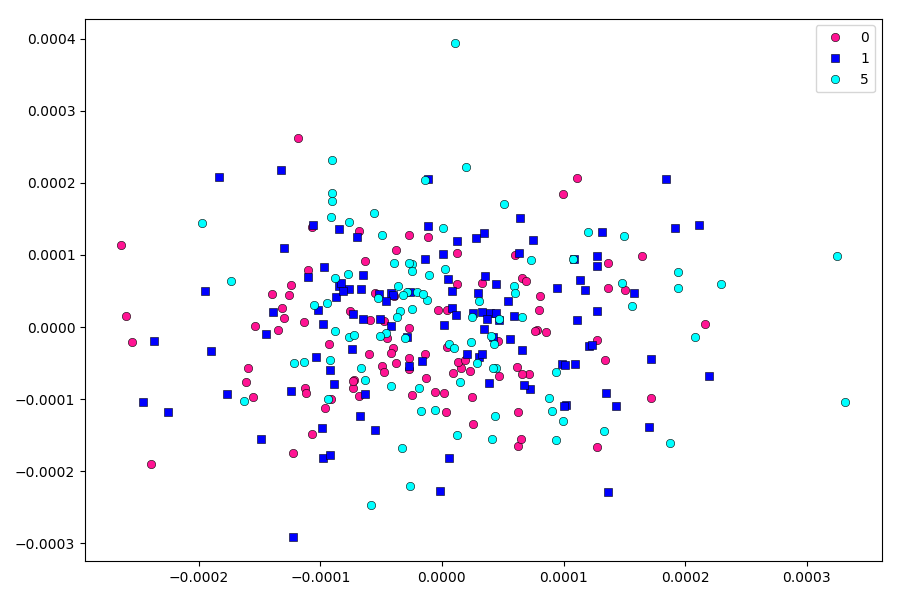
\includegraphics[width=53mm]{pics/tsne_False_iter_0.png}
}
\subfloat[10 iterations]{
  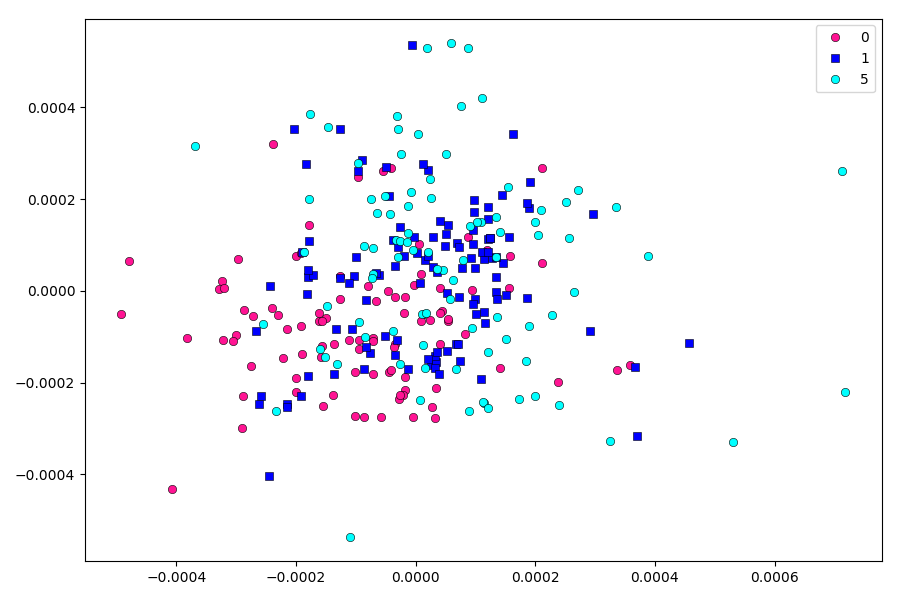
\includegraphics[width=53mm]{pics/tsne_False_iter_10.png}
}
\subfloat[20 iterations]{
  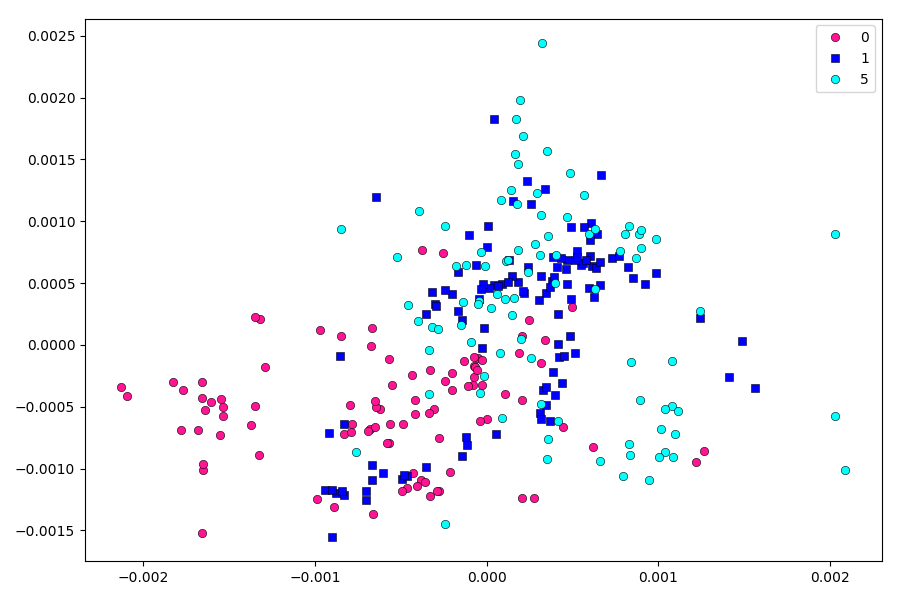
\includegraphics[width=53mm]{pics/tsne_False_iter_20.png}
}
\hspace{0mm}
\subfloat[30 iterations]{
  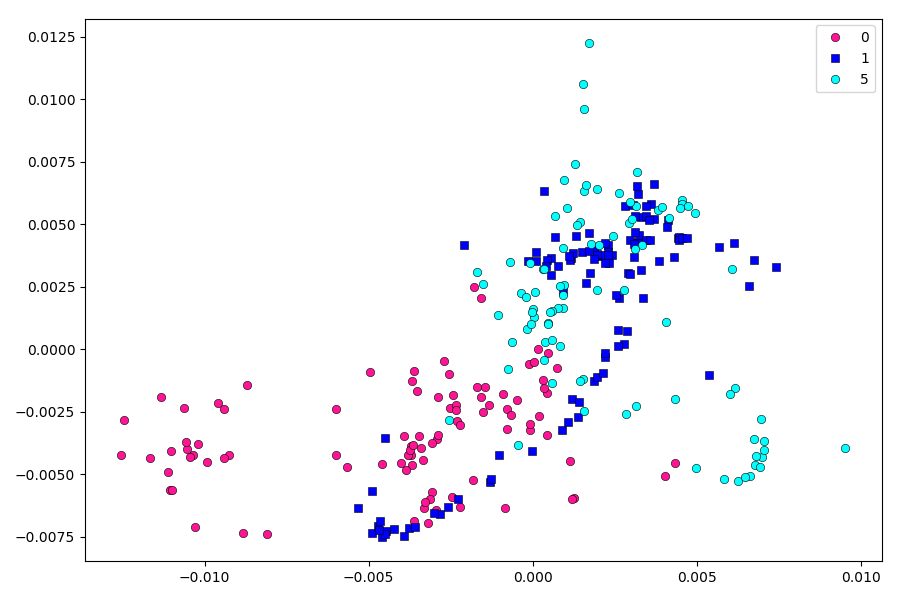
\includegraphics[width=53mm]{pics/tsne_False_iter_30.png}
}
\subfloat[40 iterations]{
  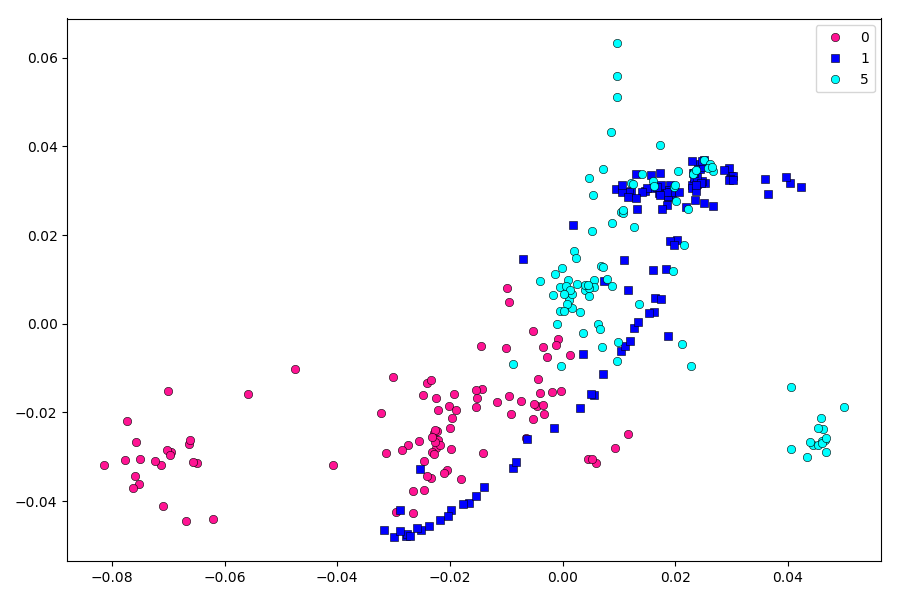
\includegraphics[width=53mm]{pics/tsne_False_iter_40.png}
}
\subfloat[50 iterations]{
  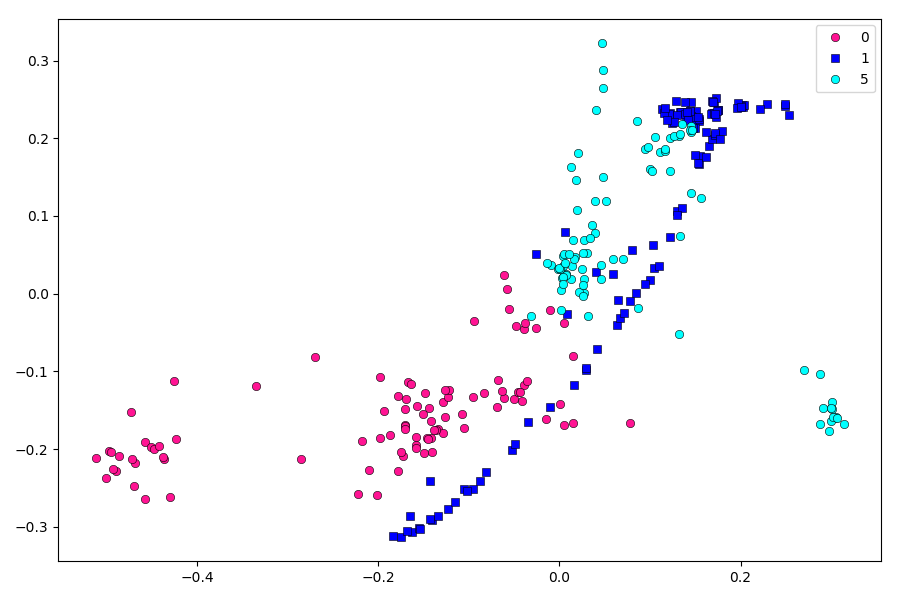
\includegraphics[width=53mm]{pics/tsne_False_iter_50.png}
}
\hspace{0mm}
\subfloat[60 iterations]{
  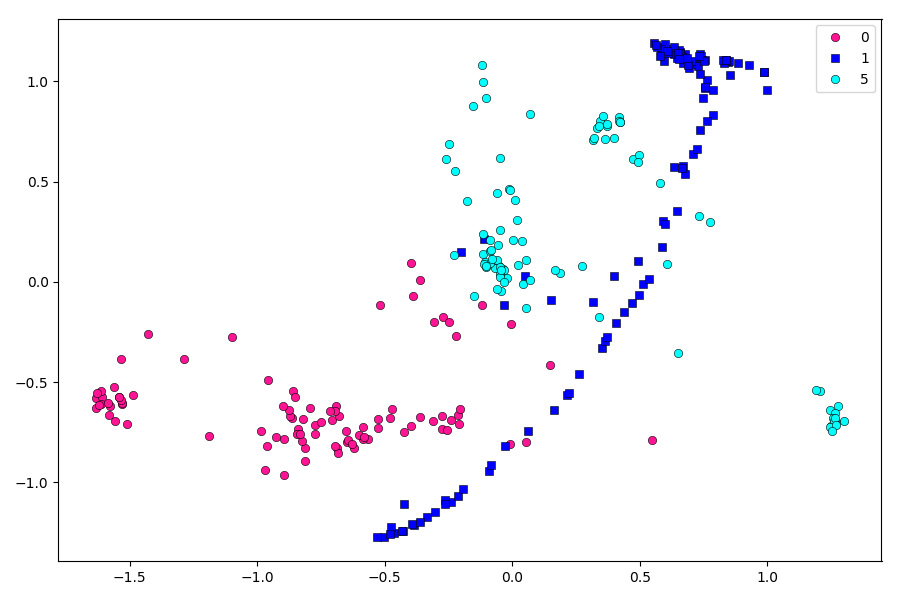
\includegraphics[width=53mm]{pics/tsne_False_iter_60.png}
}
\subfloat[70 iterations]{
  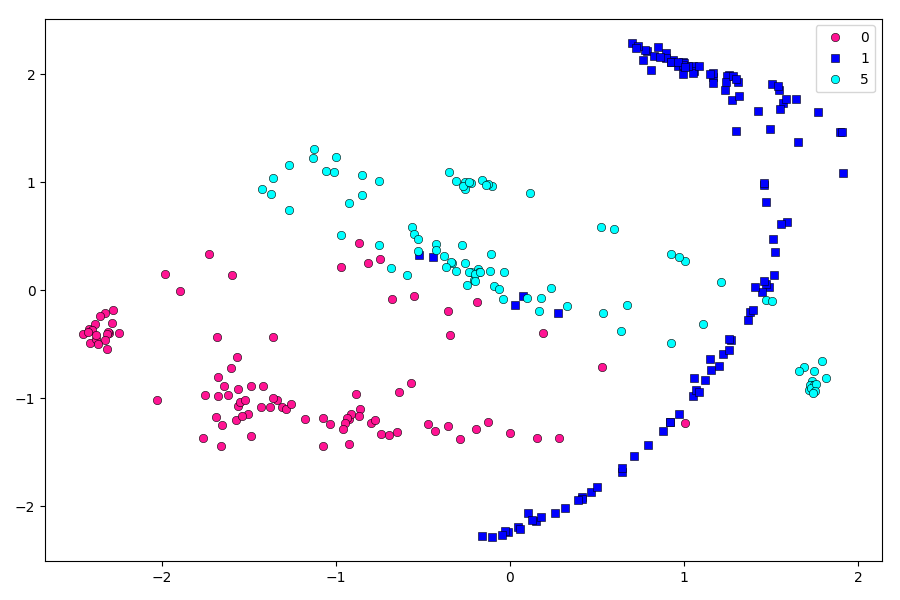
\includegraphics[width=53mm]{pics/tsne_False_iter_70.png}
}
\subfloat[80 iterations]{
  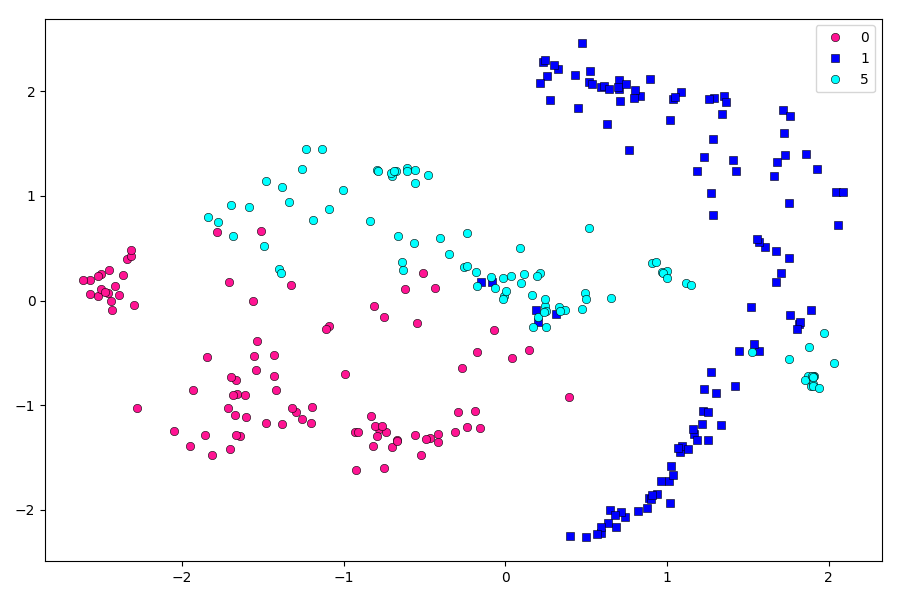
\includegraphics[width=53mm]{pics/tsne_False_iter_80.png}
}
\hspace{0mm}
\subfloat[90 iterations]{
  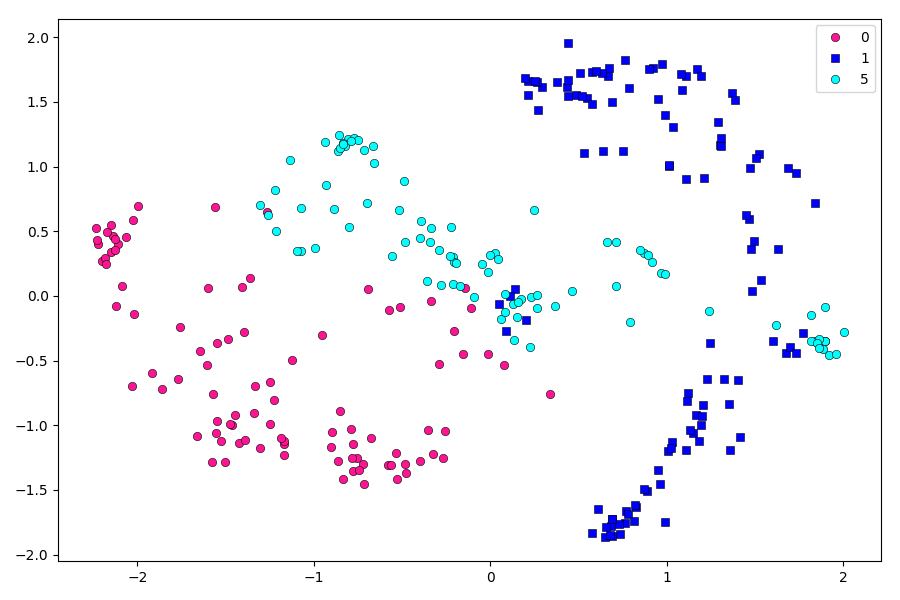
\includegraphics[width=53mm]{pics/tsne_False_iter_90.png}
}
\subfloat[100 iterations]{
  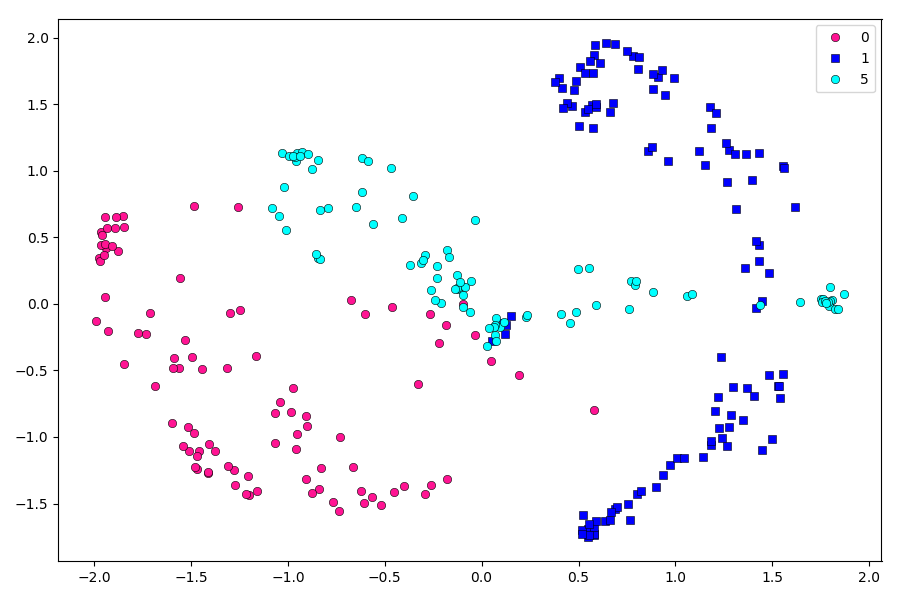
\includegraphics[width=53mm]{pics/tsne_False_iter_100.png}
}
\subfloat[110 iterations]{
  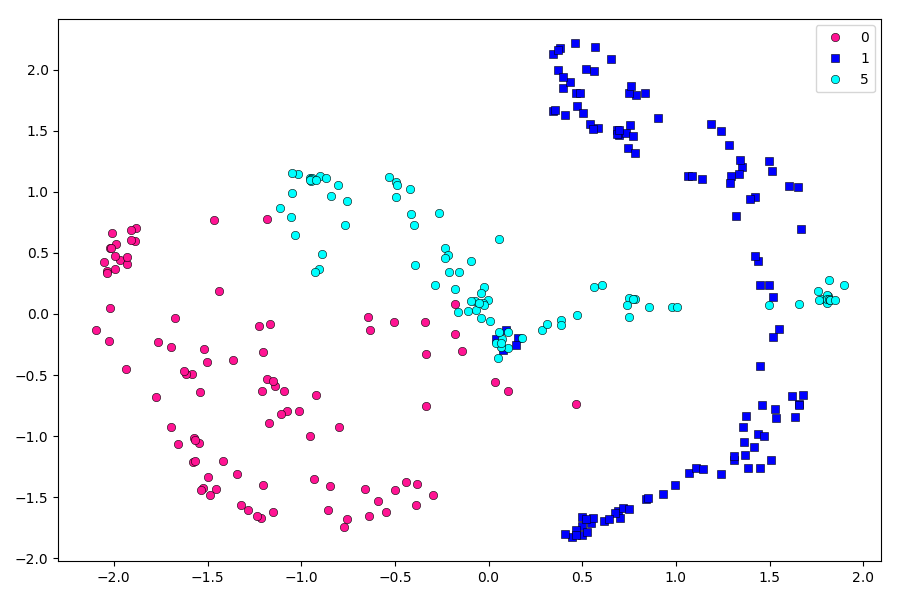
\includegraphics[width=53mm]{pics/tsne_False_iter_110.png}
}
\caption{Results of the SNE applied on the MNIST dataset}
\end{figure}

